En esta sección desarrollaremos y mostraremos los resultados de los experimentos para:

\begin{itemize}
\item Los protocolos distinguidos.
\item La incidencia de paquetes ARP en la red.
\item Los nodos distinguidos.
\end{itemize}

Para realizar estos experimentos analizaremos los siguientes datasets, cada uno tomado en circunstancias diferentes:

\begin{itemize}
\item Dataset 1: Biblioteca pabellón 2 (wifi) a las 3pm, captura de 10 minutos
\item Dataset 2: Laboratorios pabellón 1 (wifi) a las 5pm, captura de 10 minutos
\item Dataset 3: Hogar de uno de los integrantes del grupo, sin ningun otro dispositivo(wifi) a las 12am, captura de 15 minutos
\item Dataset 4: Hogar de uno de los integrantes del grupo, con más dispositivos conectados a la red(wifi) a las 12:20pm, captura de 15 minutos
\item Dataset 5: Red de un Starbucks(wifi), captura de 10 minutos
\item Dataset 6: Red de la Biblioteca Noriega del pabellón 1(wifi), captura de 30 minutos
\end{itemize}


\subsection{Experimento protocolos distinguidos}

Para analizar los protocolos distinguidos fuimos guardando los resultados de sniffear diferentes redes y tomar como fuente de información S el campo .type de los paquetes que se fueron procesando. De ahí calculamos la cantidad de apariciones de cada protocolo, la probabilidad de aparición de cada protocolo, calculamos la entropía y la comparamos con la información que aporta cada símbolo de S.\\

Ahora, para analizar los datos, planteamos histogramas donde podemos ver la cantidad de información que aporta cada símbolo de la fuente. Luego lo comparamos con la entropía y definimos los \textbf{protocolos distinguidos} como los que son mas bajos que la entropía. Esto lo hicimos porque según lo que explicamos en la introducción, los símbolos cuya cantidad de información es mas baja que la entropía son muy predecibles y aparecerán muchas veces. \\

Los resultados fueron los siguientes: \\

% Dataset 1 ----------------------------------

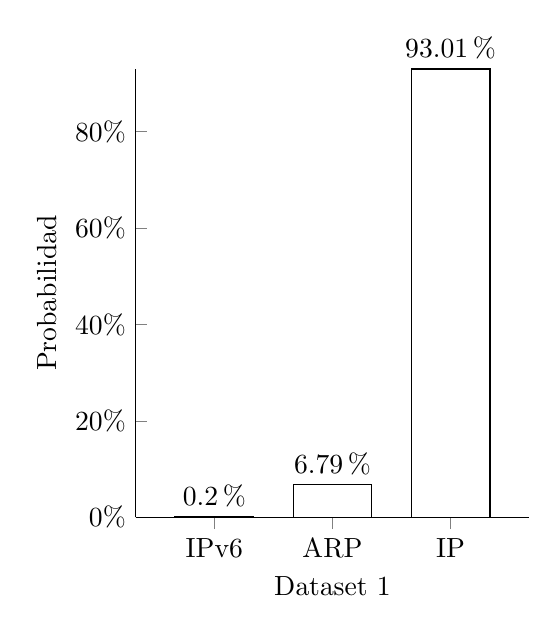
\begin{tikzpicture}
\begin{axis}[
    ybar,
    bar width=1cm, % Width of the bar
    x=1.5cm, % Distance between the centers of the bars
    enlarge x limits={abs=1cm}, % The distance between the center of the first bar and the left edge
    enlarge y limits=false,
    ymin=0,
    xtick=data,
    xlabel= {Dataset 1},
    ylabel= {Probabilidad},
    symbolic x coords={IPv6,ARP,IP},
    point meta={y*100}, %y-Werte mal 100 für Prozent
    yticklabel={\pgfmathparse{\tick*100}\pgfmathprintnumber{\pgfmathresult}\%},
    axis lines*=left,
    clip=false
    ]
\addplot [
    draw=black,
    fill=white,
    nodes near coords={\pgfmathprintnumber{\pgfplotspointmeta}\,\%},
    error bars/.cd,
        y dir=both,
        y explicit
    ] coordinates{(IPv6,0.001998001998)
        (ARP,0.0679320679321)
        (IP,0.93006993007)};
\end{axis}
\end{tikzpicture}
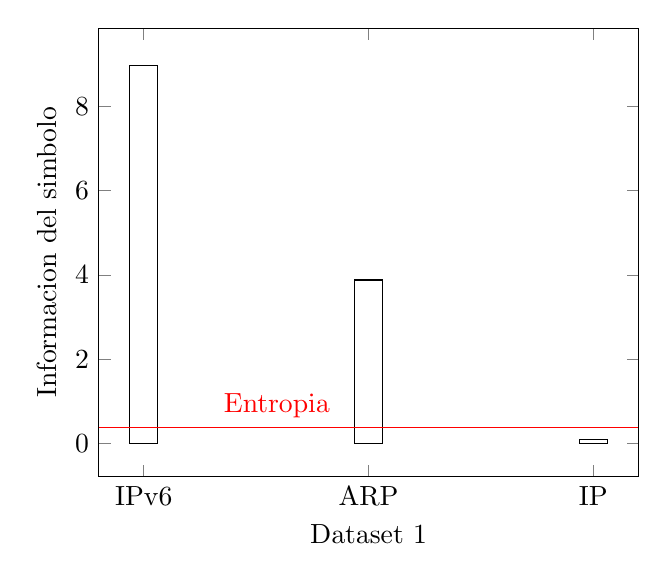
\begin{tikzpicture}
\begin{axis}[
    symbolic x coords={IPv6,ARP,IP},
        ylabel = {Informacion del simbolo},
        xlabel = {Dataset 1},
        xtick=data]
    \addplot[ybar,fill=white] coordinates {
        (IPv6,8.9672262584)
        (ARP,3.8797634179)
        (IP,0.1045889014)
    };
    \draw [red] ({rel axis cs:0,0}|-{axis cs:ARP,0.378751880122}) -- ({rel axis cs:1,0}|-{axis cs:ARP,0.378751880122}) node [pos=0.33, above] {Entropia};
\end{axis}
\end{tikzpicture} \\

% Dataset 2 ----------------------------------

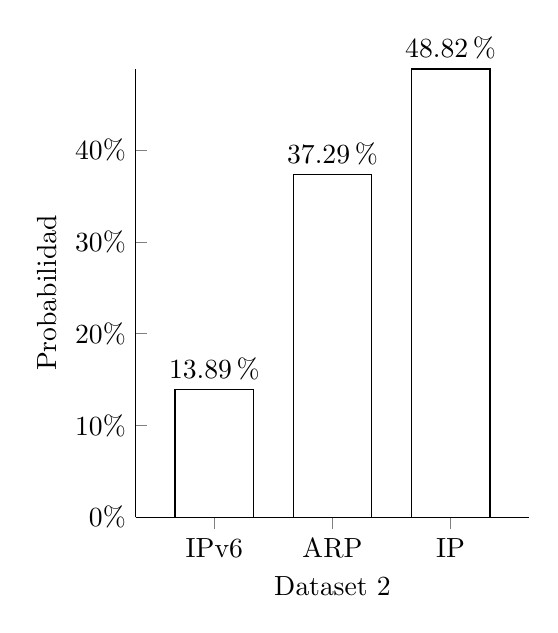
\begin{tikzpicture}
\begin{axis}[
    ybar,
    bar width=1cm, % Width of the bar
    x=1.5cm, % Distance between the centers of the bars
    enlarge x limits={abs=1cm}, % The distance between the center of the first bar and the left edge
    enlarge y limits=false,
    ymin=0,
    xtick=data,
    xlabel= {Dataset 2},
    ylabel= {Probabilidad},
    symbolic x coords={IPv6,ARP,IP},
    point meta={y*100}, %y-Werte mal 100 für Prozent
    yticklabel={\pgfmathparse{\tick*100}\pgfmathprintnumber{\pgfmathresult}\%},
    axis lines*=left,
    clip=false
    ]
\addplot [
    draw=black,
    fill=white,
    nodes near coords={\pgfmathprintnumber{\pgfplotspointmeta}\,\%},
    error bars/.cd,
        y dir=both,
        y explicit
    ] coordinates{
        (IPv6,0.1389218889)
        (ARP,0.3728838729)
        (IP,0.4881942382)};
\end{axis}
\end{tikzpicture}
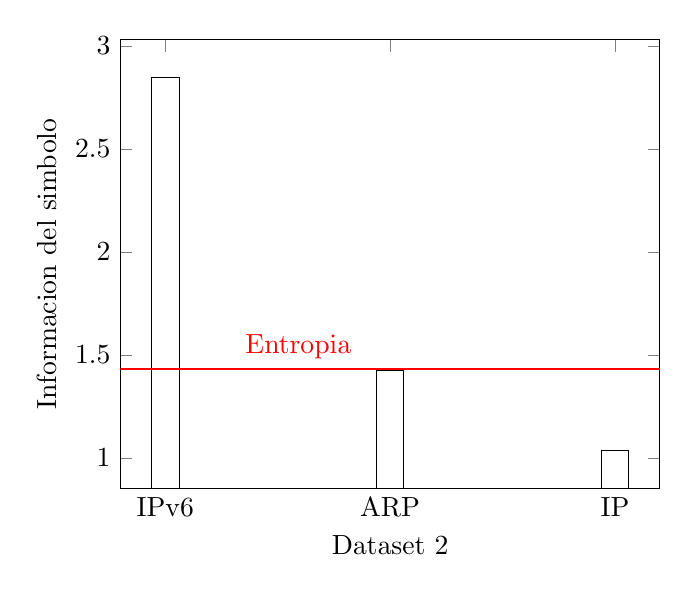
\begin{tikzpicture}
\begin{axis}[
    symbolic x coords={IPv6,ARP,IP},
        ylabel = {Informacion del simbolo},
        xlabel = {Dataset 2},
        xtick=data]
    \addplot[ybar,fill=white] coordinates {
        (IPv6,2.847654163)
        (ARP,1.423201692)
        (IP,1.034472826)
    };
    \draw [red] ({rel axis cs:0,0}|-{axis cs:ARP,1.4313141279}) -- ({rel axis cs:1,0}|-{axis cs:ARP,1.4313141279}) node [pos=0.33, above] {Entropia};
\end{axis}
\end{tikzpicture} \\

% Discusion ------------------------------------

Por lo que podemos ver, la incidencia de ARP es muy baja en el Dataset 1 ya que en una biblioteca hay poco recambio de dispositivos y pocos hosts, lo cual hace que la incidencia de ARP sea menor. En cambio, si hay muchos mas paquetes IP, lo cual tiene sentido porque es el protocolo que todos los hosts usan para conectarse a internet. Entonces como podemos ver, el único símbolo predecible menor que la entropía es el de IP, el cual es el único protocolo distinguido en este dataset. \\

En el segundo Dataset, ya podemos hablar de una red (el Laboratorio de Computación) en la cual no solamente hay muchos mas hosts, sino el recambio de dispositivos que entran y se van de la red es mayor, por lo cual la incidencia de ARP sube. A su vez, IP sigue siendo el protocolo más usado al igual que en el dataset anterior. Tanto la información que aporta ARP como IP superan la entropía de la fuente de información S, por eso ambos son en este caso protocolos distinguidos. \\
% end subsection

\subsection{Experimento incidencia de ARP}

Usaremos la misma forma de medir que describimos en el ejercicio anterior para poder observar la incidencia de paquetes ARP en la red voy a utilizar una serie de muestras
tomadas de distintas redes y graficarlas en un histograma, después de mostrar los resultados daremos una explicación del por que de los mismo. Aclaración: todas las capturas
son de 15 minutos.

\begin{figure}[H]
\centering
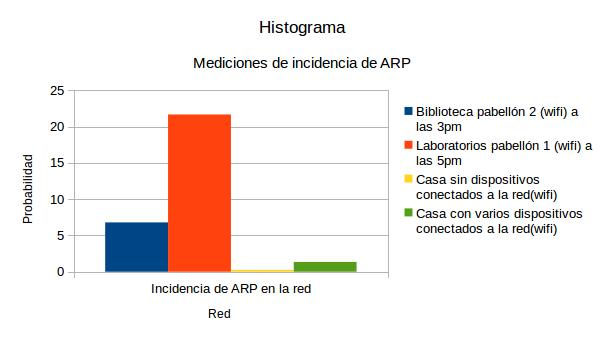
\includegraphics[width=90mm]{imagenes/IncidenciaARP.jpg}
\caption{Comparación de porcentaje de apariciones de ARP en distintas redes o con distintas condiciones.\label{overflow}}
\end{figure}

Como podemos ver la red de los laboratorios tiene más porcentaje de paquetes ARP que el de la biblioteca. Esto se debe a que en el laboratorio del pabellón 1 ingresan
constantemente personas y, por lo tanto, la mayoría de ellos ingresan en la red a través de las computadoras del mismo o usando el wifi de estos con sus celulares. Esto
ocurre en menor medida en la biblioteca ya que no se usan computadoras que no sean propias de los que ingresan y, por lo tanto, hay mucho más tráfico de paquetes ARP en la red
de los laboratorios. Además al estar en una red privada, es más común que se efectúen envíos de mensajes entre computadoras y los routers de las mismas.\\

En menor medida tenemos los casos tomados en la red de un hogar, teniendo como sus dos mediciones a cuando solamente hay un dispositivo, el mismo con el que se realiza la medición,
conectado a la red y cuando hay más cantidad. Podemos ver que el tráfico de paquetes ARP es muy bajo en ambos casos en comparación a las muestras anteriores. Sin embargo,
cuando hay mayor cantidad de dispositivos el tráfico general aumenta y también el porcentaje de paquetes ARP, porque en este caso hay mas hosts.\\

Por último tenemos dos mediciones realizadas en la biblioteca Noriega y un Starbucks, en estas podemos ver resultados similares a los anteriores. La biblioteca tiene a muchas
gente entrando y saliendo, muchos de ellos se quedan a usar las instalaciones para estudiar con sus celulares y computadoras portatiles. En el Starbucks notamos que era menos
común cuando se realizo las mediciones.\\

La conclusión que podemos sacar es que si bien estas muestras pertenecen a distintos lugares y horarios podemos ver como el tráfico de paquetes ARP es más significativo cuando 
la red tiende a obtener nuevos hosts con más constancia.

% end subsection


\subsection{Experimento nodos distinguidos}

Para distinguir los nodos de una red, analizaremos la \texttt{IP} fuente y destino de los paquetes \texttt{ARP Who-Has}.
No utilizaremos otros paquetes distintos de \texttt{ARP}, ya que queremos restringirnos a las comunicaciones internas de la subred.

\begin{itemize}
    \item Diremos que un nodo es \textbf{distinguido como destino}, si la probabilidad de que sea destino en un paquete \texttt{Who-Has} es alta (que signfica alta?).

        En esta categoria, podríamos conjeturar que el Gateway de una red va a ser un nodo distinguido como destino,
        ya que los otros nodos buscan enviarle información a su IP constantemente.
    \item Diremos que un nodo es \textbf{distinguido como fuente}, si la probabilidad de que sea fuente en un paquete \texttt{Who-Has} es alta (que signfica alta?).

        En esta categoria, un nodo tendría que enviar muchos más paquetes que el resto para distinguirse como fuente.
\end{itemize}
